\documentclass[./main.tex]{subfiles}
\begin{document}
\begin{subappendices}

\chapter{Inmunomarcación de células mutantes estimuladas con diferentes dosis de FGF4}
\chaptermark{Inmunomarcación de células mutantes...}
\label{C3_ap:inmuno}

Nos preguntamos si la variabilidad de la activación de ERK en células individuales que observamos en el capítulo \ref{ch2} se conservaba para esta condición experimental, en donde eramos capaces de controlar la dosis de estímulo extracelular a partir de estimular mESCs mutantes en \textit{Fgf4} (figura \ref{C2_fig:inmuno}). Para responder a este interrogante, realizamos una inmunomarcación para distintas concentraciones de FGF4 en el rango que elegimos para estimular las células. En la figura \ref{C3_fig:FGF_inmuno}A observamos que los niveles de pERK aumentaban conforme a la concentración de FGF4 extracelular, pero la variabilidad que observamos en las células \textit{wild type} en s+L se conservaba. Este resultado fue comprobado en la cuantificación que exponemos en la figura \ref{C3_fig:FGF_inmuno}B. Esta cuantificación reveló que la mediana y los valores más bajos aumentaban conforme a la dosis de FGF4, al igual que la varianza. Estos resultados sugieren que la variabilidad de la activación de ERK en ESCs individuales no es producto de mantener a las células en condiciones de cultivo químicamente indefinidas, sino que probablemente sea producto de mecanismos intracelulares. 



\begin{figure}
    \centering
    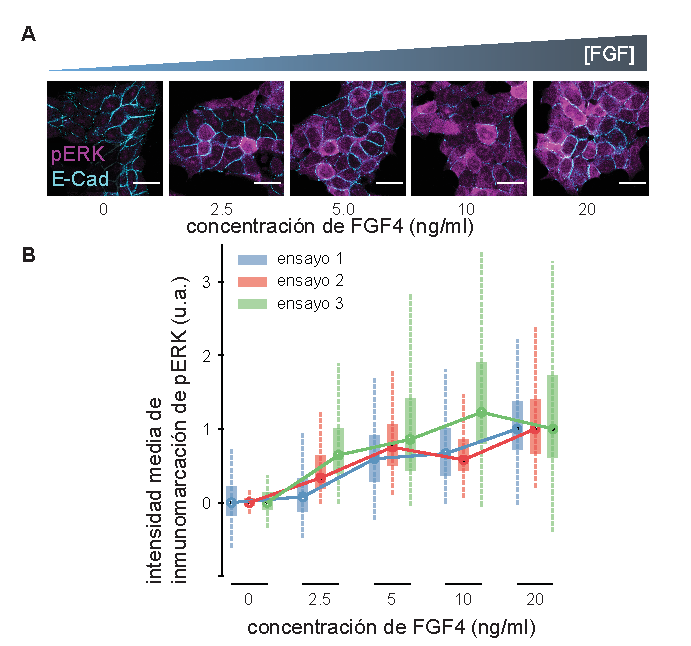
\includegraphics[width=1\columnwidth]{figures/chapter3/C3_FGF_inmuno.pdf} 
    \caption{\textbf{Distribución de los niveles de pERK de células individuales estimuladas con diferentes dosis de FGF4.} (A) Inmunomarcación de células mutantes de \textit{Fgf4} para pERK (magenta) y E-Cadherina (cian) para delinear los límites celulares. Las células fueron tratadas con las concentraciones indicadas de FGF4. Las células pretrataron con  N2B27 + chiron + LIF y FGF4 por 24 horas, y 4 horas antes de la medición se repuso el medio, pero sin LIF. Barra de escala = 20 $\mu m$. (B) \textit{Boxplots} de la intensidad de pERK en células individuales para tres ensayos diferentes, teñidos como en B. Los círculos indican la mediana, las cajas sólidas el rango intercuartil, los bigotes son 1,5 veces el rango intercuartil. En cada ensayo, primero se restó la mediana de la condición de $0$ ng/ml de todas las mediciones de células individuales, y luego se normalizó a la mediana de la condición de $20$ ng/ml. Los detalles del experimento se encuentran en \cite{Fabris2022}.}
    \label{C3_fig:FGF_inmuno}
\end{figure}

\chapter{Detalles de la implementación de la detección de pulsos en series temporales experimentales de actividad de ERK de alta resolución temporal}
\chaptermark{Detección de pulsos}

\section{Detección de pulsos en series temporales extraídas de células mutantes estimuladas con FGF4}
\sectionmark{Detección de pulsos en mutantes estimuladas con FGF4}
\label{C3_ap:FGF_pulse_detection}


Empleamos una estrategia similar a la descripta en la sección \ref{C2_sec:pulse_detection} para distinguir pulsos de fluctuaciones de base en las series temporales de la figura \ref{C3_fig:FGF_traces}. Durante el preprocesamiento de las señales, eliminamos los últimos 20 cuadros de las series temporales de las células 15, 27 y 32 (0 ng/ml), 14, 20, 34, 38, 41, 43 y 44 (2,5 ng/ml), 13 (5 ng/ml), y 8 y 39 (20 ng/ml). 

Para el algoritmo de detección, establecimos los parámetros umbrales entendiendo a la condición no tratada como la condición donde esperábamos no detectar pulsos de ERK, y la condición de $20$ ng/ml como la condición en donde esperábamos que ERK esté más activo (figura \ref{C3_ap_fig:FGF_pulse_detection}). Los valores de los parámetros se encuentran en la cuadro \ref{C3_ap_tab:FGF_th}.

\begin{figure}
    \centering
    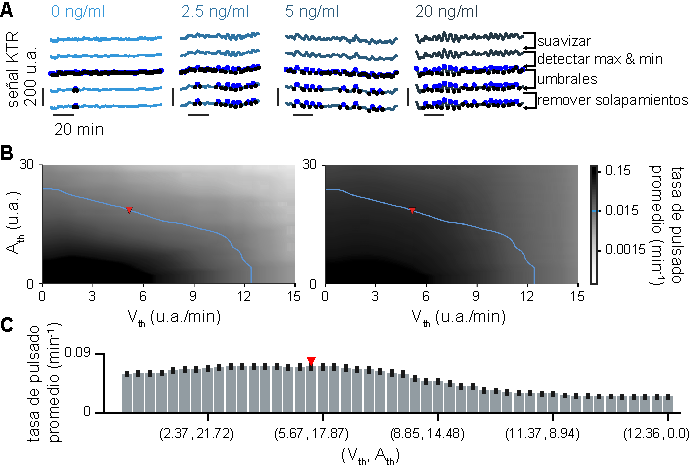
\includegraphics[width=1\columnwidth]{figures/chapter3/C3_FGF_pulse_detection.pdf}\caption{\textbf{Protocolo de reconocimiento de pulsos y análisis de umbrales en el experimento de estimulación controlada de FGF4.} (A) Series temporales representativas de la actividad dinámica de ERK en células mutantes en el gen \textit{Fgf4} estimuladas con diferentes dosis de FGF4 (columnas), codificadas en colores como en la figura \ref{C3_fig:FGF_traces}B. Las filas ilustran los pasos del algoritmo de reconocimiento de pulsos: la primera fila muestra los datos crudos, la segunda muestra las series temporales suavizadas. Los puntos azules y negros de la tercera fila son máximos y mínimos locales. La cuarta fila muestra los máximos y mínimos locales que superan los umbrales de amplitud y pendiente. La quinta, muestra los pulsos identificados tras eliminar los solapamientos. Los pulsos están definidos por los máximos y sus mínimos adyacentes. (B) Tasa media de pulsado en función de los umbrales de amplitud y pendiente para las células mutantes en \textit{Fgf4} sin estímulo (izquierda) o con 20 ng/ml de FGF4 (derecha). La curva de nivel en la que la tasa media de pulsado en las células sin estimular es de $0.015 \;\text{min}^{-1}$ (línea azul) se utilizó para explorar combinaciones de valores de umbral de amplitud y pendiente en la condición estimulada con 20 ng/ml de FGF4. (C) Tasa media de pulsado para combinaciones de umbrales de amplitud y pendiente a lo largo de la curva azul de B en células mutantes en FGF4 estimuladas con 20ng/ml de FGF4. La barra de error indica la desviación estándar dividido la raíz cuadrada del tamaño de la muestra. El triángulo rojo en B,C indica los valores de los parámetros utilizados para el análisis posterior (cuadro \ref{C3_ap_tab:FGF_th}).}
    \label{C3_ap_fig:FGF_pulse_detection}
\end{figure}

\begin{table}[htbp]
\begin{adjustwidth}{-0.5in}{-0.5in}% adjust the L and R margins by 1 inch
\centering
\begin{tabular}{|l|l|l|l|l|l|l|}
\hline
 control & control & espacio & curva & umbral & umbral \\
 negativo & positivo & exploratorio & de nivel ($\delta_p^*$) & de & de \\
 &  & de parámetros & & amplitud & pendiente \\
\hline \hline
0 ng/ml FGF4 & 20 ng/ml FGF4 & $v_{\text{th}}$ : (0,15) $\frac{\text{u.a.}}{\text{min}}$ & $15 \times 10^{-3} \frac{1}{\text{min}}$ & 18.47 u.a. & $5.16$ $\frac{\text{u.a.}}{\text{min}}$ \\
 & & de res.: $0.5 \frac{\text{u.a.}}{\text{min}}$ & & & \\
 & & $A_{\text{th}}$ : (0,40) u.a. & & & \\
 & & res: 1 u.a. & & & \\
\hline
\end{tabular}
\end{adjustwidth}
\caption{Parámetros del algoritmo de detección de pulsos que surgieron del protocolo de análisis de umbrales para las series temporales de la figura \ref{C3_fig:FGF_traces} que describen la actividad dinámica de ERK en mESCs con una mutación de pérdida en el gen \textit{Fgf4} estimuladas con distintas dosis de FGF4 exógeno.}
\label{C3_ap_tab:FGF_th}
\end{table}

\section{Distribución de amplitud de pulsos de series temporales extraídas de células mutantes estimuladas con FGF4}
\sectionmark{Distribución de amplitud}
\label{ap_C3:amplitud}

Presentamos la distribución de amplitudes de pulsos que obtuvimos para cada condición experimental con dosis definidas de FGF extracelular en la figura \ref{C3_fig:FGF_amplitud}. En el caso donde las células mutantes no fueron estimuladas con FGF4 no había suficiente estadística y decidimos no incluirla en el análisis. A simple vista, las distribuciones de amplitudes no parecían presentar diferencias importantes. Para formalizar esta observación, implementamos el test de Kolmogorov-Smirnov para dos muestras para comparar las distribuciones de amplitud entre sí, y comprobamos que las distribuciones de amplitud no eran significativamente diferentes entre las tres concentraciones estudiadas (ver cuadro \ref{C3_ap_tab:KS}, apéndice \ref{C3_ap:FGF_KS_test}). 


\begin{figure}
    \centering
    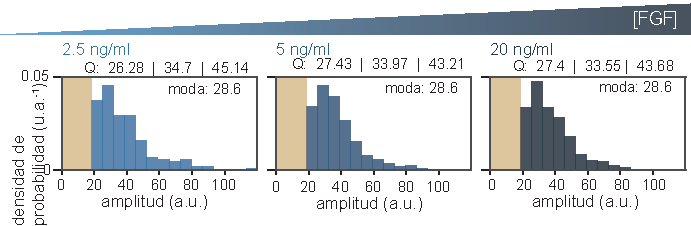
\includegraphics[width=1\columnwidth]{figures/chapter3/C3_FGF_amplitud.pdf}
    \caption{ \textbf{Distribución de las amplitudes de pulsos obtenidas en condiciones experimentales donde se estimuló con diferentes dosis de FGF4.} Distribuciones de la amplitud de los pulsos para para cada condición experimental, donde células mutantes de \textit{Fgf4} fueron estimuladas con diferentes dosis de FGF4, indicadas arriba. El número de pulsos fue n = 164 ($2.5$ ng/ml), n = 426 (5 ng/ml) y n = 544 (20 ng/ml). Se indican el límite de resolución del algoritmo de reconocimiento de pulsos (barra amarilla) y los cuartiles (Q) 25, 50 y 75. }
    \label{C3_fig:FGF_amplitud}
\end{figure}


\section{Detección de pulsos en las series temporales extraídas de los experimentos con EpiSCs}
\sectionmark{Detección de pulsos en EpiSCs}
\label{C3_ap:EPI_pulse_detection}


Empleamos una estrategia similar a la descripta en la sección \ref{C2_sec:pulse_detection} para distinguir pulsos de fluctuaciones de base en las series temporales de la figura \ref{C3_fig:EPI_traces}. Durante el preprocesamiento de las señales, eliminamos los últimos 20 cuadros de las series temporales asociadas a la célula 27 de EpiSCs en FAX, y la célula 1 de ESCs en FAX.  


Para el algoritmo de detección, establecimos un conjunto de  parámetros umbrales para cada tipo celular. Tanto para el caso de las EpiSCs como de las ESCs, consideramos a las células con MEKi como la condición donde esperábamos no detectar pulsos de ERK, y las células tratadas sólo con FAX como la condición en donde esperábamos que ERK esté más activo (figura \ref{C3_ap_fig:EPI_pulse_detection}). Los valores de los parámetros se encuentran en la cuadro \ref{C3_ap_tab:EPI_th}.

\begin{figure}
    \centering
    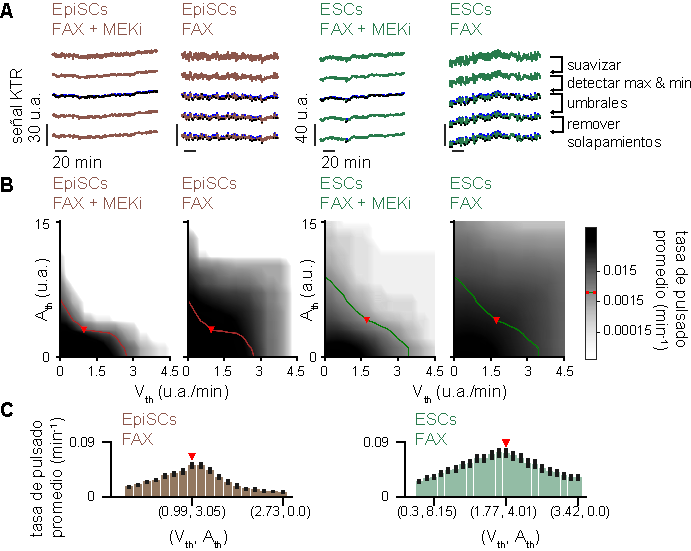
\includegraphics[width=1\columnwidth]{figures/chapter3/C3_EpiSC_pulse_detection.pdf}\caption{\textbf{Protocolo de reconocimiento de pulsos y análisis de umbrales en el experimento de EpiSCs en FAX.} 
    (A) Series temporales representativas de la actividad dinámica de ERK en EpiSCs individuales y en ESCs cultivadas en FAX con o sin MEKi (columnas), codificadas en colores como en la figura \ref{C3_fig:EPI_traces}B. Las filas ilustran los pasos del algoritmo de reconocimiento de pulsos: la primera fila muestra los datos crudos, la segunda muestra las series temporales suavizadas. Los puntos azules y negros de la tercera fila son máximos y mínimos locales. La cuarta fila muestra los máximos y mínimos locales que superan los umbrales de amplitud y pendiente. La quinta, muestra los pulsos identificados tras eliminar los solapamientos. Los pulsos están definidos por los máximos y sus mínimos adyacentes. (B) Tasa media de pulsado en función de los umbrales de amplitud y pendiente para las condiciones experimentales indicadas. Las curvas de nivel en la que la tasa media de pulsado en las células tratadas con FAX y MEKi es de $0.003 \; \text{min}^{-1}$ (linea roja para EpiSCs, linea verde para ESCs) se utilizaron para explorar combinaciones de valores de umbrales de amplitud y pendiente en las condiciones tratadas en FAX únicamente. (C) Tasa media de pulsado para combinaciones de umbrales de amplitud y pendiente a lo largo de las curvas de nivel mostradas en B para EpiSCs (izquierda) y ESCs (derecha) cultivadas sólo en FAX. La barra de error indica la desviación estándar dividido la raíz cuadrada del tamaño de la muestra. El triángulo rojo en B,C indica los valores de los parámetros utilizados para el análisis posterior (cuadro \ref{C3_ap_tab:EPI_th}).}
    \label{C3_ap_fig:EPI_pulse_detection}
\end{figure}

\begin{table}[htbp]
\begin{adjustwidth}{-0.5in}{-0.5in}% adjust the L and R margins by 1 inch
\centering
\begin{tabular}{|l|l|l|l|l|l|l|}
\hline
 control & control & espacio & curva & umbral & umbral \\
 negativo & positivo & exploratorio & de nivel ($\delta_p^*$) & de & de \\
 &  & de parámetros & & amplitud & pendiente \\
\hline \hline
EpiSCs en& EpiSCs en& $v_{\text{th}}$ : (0,15) $\frac{\text{u.a.}}{\text{min}}$ & $3 \times 10^{-3} \frac{1}{\text{min}}$ & 3.05 u.a. & $0.99$ $\frac{\text{u.a.}}{\text{min}}$ \\
 FAX + MEKi & FAX & de res.: 1.8 $\frac{\text{u.a.}}{\text{min}}$ & & & \\ 
  & & $A_{\text{th}}$ : (0,60) u.a. & & & \\
  & &  de re.s: 0.6 u.a. & & & \\
 \hline
 ESCs en& ESCs en& $v_{\text{th}}$ : (0,15) $\frac{\text{u.a.}}{\text{min}}$ & $3 \times 10^{-3} \frac{1}{\text{min}}$ & 4.06 u.a. & $1.71$ $\frac{\text{u.a.}}{\text{min}}$ \\
 FAX + MEKi & FAX & de res.: 1.8 $\frac{\text{u.a.}}{\text{min}}$ & & & \\
  & & $A_{\text{th}}$ : (0,60) u.a. & & & \\
  & &  de res.: 0.6 u.a. & & & \\
 \hline\end{tabular} 
 \end{adjustwidth}
\caption{Parámetros del algoritmo de detección de pulsos que surgieron del protocolo de análisis de umbrales para las series temporales de la figura \ref{C3_fig:EPI_traces} que surgen de medir la actividad dinámica de ERK en mEpiSCs (arriba) y mESCs (abajo) crecidas en en FAX.}
\label{C3_ap_tab:EPI_th}
\end{table}


\chapter{Test estadístico de Kolmogorov-Smirnov}
\label{C3_ap:FGF_KS_test}


Utilizamos el test de Kolmogorov-Smirnov de dos muestras (KS) para comparar las distribuciones de las medidas cuantitativas introducidas anteriormente (figuras \ref{C3_fig:FGF_amplitud}, \ref{C3_fig:EPI_activity}C, \ref{C3_fig:FGF_consecutive} A y B). Este test cuantifica si dos distribuciones son estadísticamente indistinguibles. Al ser una prueba no paramétrica, no se requieren supuestos específicos sobre las formas de las distribuciones parentales. Además, es una prueba que no asume una distribución específica, por lo que su formulación no depende de la forma de la distribución subyacente y es válida para todas las formas de distribución \cite{Frodesen1979}. 


Implementamos la prueba KS de dos muestras disponible en el módulo stats del paquete Scipy de Python \cite{Virtanen2020}. Para todas las cantidades comparadas, informamos del valor $p$ de la prueba KS de dos muestras como $K[x,y]$, donde $x$ e $y$ se refieren a las concentraciones de estimulación que etiquetan el par de distribuciones que se comparan. Los datos agregados para todas las cantidades consideradas se resumen en la cuadro \ref{C3_ap_tab:KS}.


\begin{table}[htbp]
\begin{adjustwidth}{-0.5in}{-0.5in}% adjust the L and R margins by 1 inch
\centering
\begin{tabular}{|l||l|l|l|l|}
\hline \hline
\multicolumn{5}{|c|}{tasa de pulsado} \\ \hline
X / Y & 2.5 ng & 5 ng & 20 ng & n \\ \hline
2.5 ng & 1.000 & 0.009 & 0.005 & 48 \\
5 ng & 0.009 & 1.000 & 0.727 & 57 \\
20 ng & 0.005 & 0.727 & 1.000 & 69 \\ \hline \hline
\multicolumn{5}{|c|}{duración de pulsos} \\ \hline 
X / Y & 2.5 ng & 5 ng & 20 ng & n \\ \hline
2.5 ng & 1.000 & 0.059 & 0.002 & 164 \\
5 ng & 0.059 & 1.000 & 0.340 & 426 \\
20 ng & 0.002 & 0.340 & 1.000 & 544 \\ \hline \hline
\multicolumn{5}{|c|}{amplitud} \\ \hline 
X / Y & 2.5 ng & 5 ng & 20 ng & n \\ \hline
2.5 ng & 1.000 & 0.432 & 0.586 & 164 \\
5 ng & 0.432 & 1.000 & 0.835 & 426 \\
20 ng & 0.586 & 0.835 & 1.000 & 544 \\ \hline \hline
\multicolumn{5}{|c|}{intervalo de interpulsado} \\ \hline 
X / Y & 2.5 ng & 5 ng & 20 ng & n \\ \hline
2.5 ng & 1.000 & 0.044 & < 0.001 & 124 \\
5 ng & 0.044 & 1.000 & 0.014 & 370 \\
20 ng & < 0.001 & 0.014 & 1.000 & 479 \\ \hline \hline
%\multicolumn{5}{|c|}{pulsos consecutivos} \\ \hline  -----> Lo comenté porque no tengo idea a qué se refiere con pulsos consecutivos. Creo que esto viene de un plot anterior. Imagino que ahora que tenemos el plot de trenes de pulsos no hace falta comparar estas distribuciones no?
%X / Y & 2.5 ng & 5 ng & 20 ng & n \\ \hline
%2.5 ng & 1.000 & 0.099 & 0.082 & 48 \\
%5 ng & 0.099 & 1.000 & 0.837 & 57 \\
%20 ng & 0.082 & 0.837 & 1.000 & 69 \\ \hline  \hline
\end{tabular}
\end{adjustwidth}
\caption{Valores $p$ del test de Kolmogorov-Smirnov de dos muestras, K[x,y]. El número total de puntos de datos para cada condición $n$ se indica en la columna de la derecha de la cuadro. El bajo número de pulsos en 0 ng/ml impidió el análisis estadístico de esta condición.}
\label{C3_ap_tab:KS}
\end{table}

\chapter{Análisis de dependencia de ciclo celular}

\section{Series temporales con el filtro en frecuencias alternativo}
\label{C4_ap:band_pass_filter_cell_cycle}

Empleamos una estrategia similar a la descripta en la sección \ref{C4_sec:pulse_detection} para distinguir la localización de los picos de los pulsos en las series temporales de la figura \ref{C4_fig:traces} a las que le aplicamos el filtro de frecuencias (derecha en figura \ref{C4_fig:pulse_detection}B-D). Luego, analizamos los datos conforme a lo descripto en la sección \ref{C4_sec:analisis}. Los resultados obtenidos se encuentran en la figura \ref{C4_fig:band_pass_filter_cell_cycle}.

\begin{figure}
    \centering
    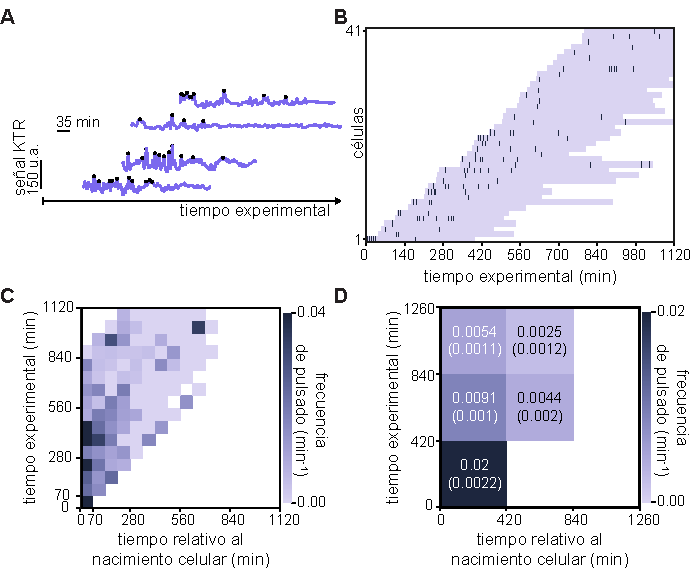
\includegraphics[width=1\columnwidth]{figures/chapter4/C4_band_pass_filter_cell_cycle.pdf}\caption{\textbf{La estrategia alternativa de filtrado en frecuencias confirma la prevalencia de la pulsación de ERK al principio del ciclo celular.} (A) Series temporales representativas de la actividad dinámica de ERK del mismo experimento reportado en la figura \ref{C4_fig:traces}, ahora implementando la estrategia alternativa de filtrado en frecuencia. Los picos identificados según el protocolo indicado de la figura \ref{C4_fig:pulse_detection} se indican como puntos negros. (B) \textit{Raster plot} que muestra la localización de los pulsos de actividad de ERK a lo largo del ciclo celular. Las bandas horizontales de color violeta se extienden desde el nacimiento hasta la división de células individuales, las barras verticales oscuras representan los picos de los pulsos. Las trazas de las células individuales comienzan inmediatamente después de la división celular y se representan en relación con el tiempo experimental absoluto. (C) Mapa de frecuencia de pulsado promediada para los datos mostrados en B. El tiempo está discretizado en intervalos de 70 minutos. (D) Mapa de frecuencia de menor resolución que muestra la frecuencia de pulsado media y su error estimado entre paréntesis. El tiempo está discretizado en intervalos de 420 minutos.}
    \label{C4_fig:band_pass_filter_cell_cycle}
\end{figure}



\section{Series temporales de células crecidas en serum + LIF}
\sectionmark{Dependencia de ciclo celular en ESCs en serum + LIF}
\label{C4_ap:s+L_cell_cycle}

Analizamos los datos de la figura \ref{C4_fig:traces} para el caso de células crecidas en serum + LIF conforme a lo descripto en la sección \ref{C4_sec:analisis}. Los resultados obtenidos luego de aplicar el filtro de linea de base a las series temporales se encuentran en la figura \ref{C4_fig:s+L_cell_cycle}.


\begin{figure}
    \centering
    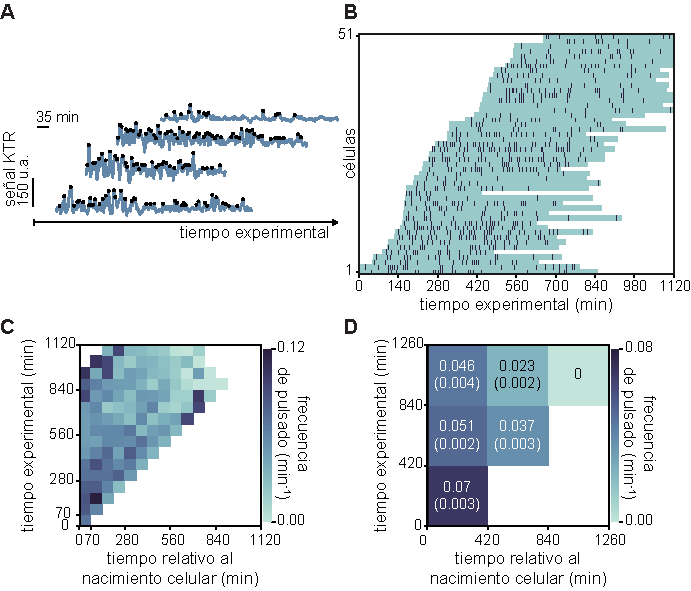
\includegraphics[width=1\columnwidth]{figures/chapter4/C4_s+L_cell_cycle.pdf}\caption{\textbf{ Los pulsos de ERK son más frecuentes al comienzo del ciclo celular en células que crecen en serum + LIF.} (A) Series temporales representativas de la actividad dinámica de ERK con picos identificados (puntos negros) en células de tipo \textit{wild type} que crecen en serum + LIF. El protocolo experimental y la estrategia de filtrado de línea de base son los mismos que en las figuras \ref{C4_fig:traces} y \ref{C4_fig:pulse_detection}. (B) \textit{Raster plot} que muestra la localización de los pulsos de actividad de ERK a lo largo del ciclo celular. Las bandas horizontales de color verde se extienden desde el nacimiento hasta la división de células individuales, las barras verticales azules oscuras representan los picos de los pulsos. Las trazas de las células individuales comienzan inmediatamente después de la división celular y se representan en relación con el tiempo experimental absoluto. (C) Mapa de frecuencia de pulsado promediada para los datos mostrados en B. El tiempo está discretizado en intervalos de 70 minutos. (D) Mapa de frecuencia de menor resolución que muestra la frecuencia de pulsado media y su error estimado entre paréntesis. El tiempo está discretizado en intervalos de 420 minutos.}
    \label{C4_fig:s+L_cell_cycle}
\end{figure}


\chapter{Detalles del cálculo analítico de la duración de pulsos}
\label{C6_ap:Txi_LI2_S2}

Corroboramos el límite \ref{C6_eq:Txi_LI2_S2} resolviendo numéricamente el comportamiento de \ref{C6_eq:Txi_LI2_S1} en un entorno de \xxi. El resultado se encuentra en la figura \ref{C6_fig:Txi_LI2_S2}. 

\begin{figure}
    \centering
    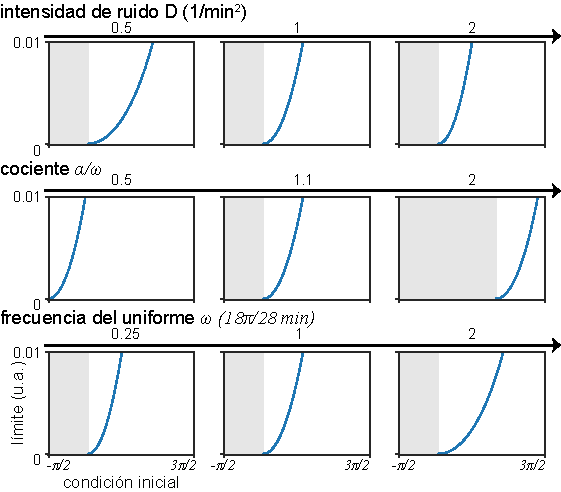
\includegraphics[width=1\columnwidth]{figures/chapter6/C6_limite_int_2.pdf} 
    \caption{\textbf{Comportamiento del término \ref{C6_eq:Txi_LI2_S1} cerca del punto fijo inestable}. Comportamiento de \ref{C6_eq:Txi_LI1} cerca del punto fijo inestable \xxi para distintos valores de la intensidad del ruido $D$, cociente adimensional $\alpha/\omega$ y frecuencia del homogéneo $\omega$ indicados. $\omega = 2\pi/7 \;\text{min}^{-1}$, $\dddelta = 1.1$ , y $\D = 1 \;\text{min}^{-2}$, a excepción de que se especifique otro valor. Los bordes de la región gris indican el punto fijo inestable si corresponde.}
    \label{C6_fig:Txi_LI2_S2}
\end{figure}

\chapter{Simulaciones numéricas de series temporales y detección de pulsos}
\label{C6_ap:traces}
\label{C7_ap:OU_OUD_traces}

Para generar numéricamente las trayectorias del modelo de fase de bifurcación de ciclo infinito con ruido blanco gaussiano de la ecuación \ref{C6_eq:adler_white_noise} implementamos el algoritmo de Heun de \cite{SanMiguel2000}. Para generar numéricamente las trayectorias de la amplitud de modulación como proceso de Ornstein-Uhlenbeck, implementamos el algoritmo de Heun de \cite{SanMiguel2000}. Para generar las trayectorias de la fase en donde la amplitud de modulación incorpora ruido de color, tanto en la sección \ref{C7_sec:OU} como en \ref{C7_sec:OUD} donde incorporamos ruido blanco aditivo, utilizamos el método de Runge-Kutta que implementa ideas similares al método de Heun descripto en \cite{SanMiguel2000}. Este enfoque es un poco más costoso computacionalmente, pero tiene la ventaja converger correctamente al ruido blanco gaussiano para valores pequeños de tiempo de retorno.


En todos los casos, para generar números aleatorios utilizamos el método de Box-Muller-Wiener. Generamos las series temporales $x(t)$ con un paso o frecuencia de sampleo de $dt$ por un total de $T$ minutos, y $n = T/dt $ pasos. Adquirimos puntos de la trayectoria de $x(t)$ cada $d$ pasos. Por lo general, las condiciones iniciales fueron sampleadas de una distribución uniforme $U(0,2\pi)$, al menos que se indique lo contrario. En el caso de la amplitud de modulación, cuando era descripta como un proceso Ornstein-Uhlenbeck su condición inicial fue su valor medio $\alpha_0$.


En todas series temporales simuladas, para detectar pulsos utilizamos el algoritmo descripto en la sección \ref{C6_ssec:deteccion_de_pulsos}. En los modelos de fase con la amplitud de modulación como proceso de OU de las secciones \ref{C7_sec:OU} y \ref{C7_sec:OUD}, consideramos a los puntos fijos como los correspondientes al valor medio de la amplitud de modulación $\alpha_0$.



\chapter{Especificaciones de la implementación del ABC-SMC}
\label{C6_ap:ABC-SMC}
\label{C7_ap:ABC-SMC}

Como \textit{prior} propusimos la siguiente distribución uniforme
\begin{equation*}
    \Pi(x) = \left\{ \begin{array}{lcc}
             \frac{1}{b-a} &   \text{si}  & x \in [a,b] \\
             \\ 0 &  \text{si} & x < a \; \text{o} \; x > b.
             \end{array}
   \right.
\end{equation*}
Los límites $a$ y $b$ de cada uno de los parámetros fueron elegidos previa inspección visual del sistema dinámico. Una correcta elección de estas funciones agiliza la convergencia del algoritmo, siendo posible que durante las iteraciones se recorran parámetros que inicialmente no están contemplados en estas \textit{prior}. 

En la sección \ref{C6_sec:alder_ruido_fit}, para la frecuencia del uniforme $\omega$, $a = \pi/14 \; \text{min}^{-1}$ y $b =  8\pi/7 \; \text{min}^{-1}$. Para el cociente adimensional \dddelta, $a = 0$ y $b = 2$. Para la intensidad de ruido $D$, $a = 0$ y $b = 2 \; \text{min}^{-2}$. En la sección \ref{C7_sec:OU}, para la frecuencia del uniforme $\omega$, $a = \pi/14 \; \text{min}^{-1}$ y $b =  8\pi/7 \; \text{min}^{-1}$. Para el cociente adimensional $\alpha_0/\omega$, $a = 0$ y $b = 2$. Para el tiempo de reversión $\tau$, $a = 1$ y $b = 200$ minutos, y para la volatilidad $\sigma$, $a = 0$ y $b = 3 \; \text{min}^{-3/2}$. En la sección \ref{C7_sec:OUD}, para la frecuencia del uniforme $\omega$, $a = \pi/14 \; \text{min}^{-1}$ y $b =  8\pi/7 \; \text{min}^{-1}$. Para el cociente adimensional $\alpha_0/\omega$, $a = 0$ y $b = 2$. Para el tiempo de reversión $\tau$, $a = 1$ y $b = 200$ minutos. Para la volatilidad $\sigma$, $a = 0$ y $b = 3 \; \text{min}^{-3/2}$, y para la intensidad de ruido $D$, $a = 0$ y $b = 2\; \text{min}^{-2}$. En la sección \ref{C7_sec:dist}, para la frecuencia del uniforme $\omega$, $a = \pi/14 \; \text{min}^{-1}$ y $b =  8\pi/7 \; \text{min}^{-1}$. Para el cociente adimensional $\mu_{\alpha}/\omega$, $a = 0$ y $b = 2$. Para la desviación estándar normalizada $\sigma_{\alpha}/\omega$, $a = 0$ y $b = 5$, y para la intensidad de ruido $D$, $a = 0$ y $b = 2\; \text{min}^{-2}$.


En las secciones \ref{C6_sec:alder_ruido_fit}, \ref{C7_sec:OU} y \ref{C7_sec:OUD} cada serie temporal simulada durante la implementación del algoritmo tenía una frecuencia de sampleo $dt = 0.001 \text{ min}$, una frecuencia de adquisición de $d = 1$ paso y una duración total de $T = 1000 \text{ min}$. Para calcular la distribución de duración de pulsos de cada serie temporal, utilizamos el algoritmo de detección de pulsos descripto en la sección \ref{C6_ssec:deteccion_de_pulsos}, con un umbral de amplitud $A_{\text{th}} = 0.9$ y una distancia umbral $W_{\text{th}} = 100 \text{ cuadros}$. También utilizamos el resultado de implementar este algoritmo para estimar la la mediana de la tasa de pulsado como cantidad de pulsos detectados sobre $T = 1000 \text{ min}$. Para obtener la distribución de intervalo de interpulsado, utilizamos el procedimiento descripto en la sección \ref{C6_ssec:deteccion_de_pulsos}.  


En la sección \ref{C7_sec:dist} cada serie temporal simulada durante la implementación del algoritmo tenía una frecuencia de sampleo $dt = 0.001 \text{ min}$, una frecuencia de adquisición de $d = 1$ paso y una duración total de $T = 100 \text{ min}$. En cada evaluación simulamos $30$ series temporales con estas características, cada una con una amplitud de modulación distinta que adquirimos de distribución de muestreo definida por los parámetros $\mu_{\alpha}$ y $\sigma_{\alpha}$. Para calcular la distribución de duración de pulsos de cada serie temporal, utilizamos el algoritmo de detección de pulsos descripto en la sección \ref{C6_ssec:deteccion_de_pulsos}, con un umbral de amplitud $A_{\text{th}} = 0.9$ y una distancia umbral $W_{\text{th}} = 100 \text{ cuadros}$ para cada una de las 30 series temporales.  Para obtener la distribución de intervalo de interpulsado,  utilizamos el procedimiento descripto en la sección \ref{C6_ssec:deteccion_de_pulsos} para cada serie temporal. Finalmente, para calculamos la tasa de pulsado de cada serie temporal, y luego tomamos su mediana. 


Durante todo este capítulo, la tolerancia mínima que determinaba el final del algoritmo fue de $\epsilon = 0.1$, que elegimos basándonos en la implementación de \cite{Costa2021}. También establecimos un número máximo de $21$ iteraciones, límite al cual no fue necesario recurrir. Las tolerancias que obtuvimos en cada una de las implementaciones de las secciones  \ref{C7_sec:OU}, \ref{C7_sec:OUD} y \ref{C7_sec:dist} se encuentran en la figura 
\ref{C7_fig:ap_eps}.

\begin{figure}
    \centering
    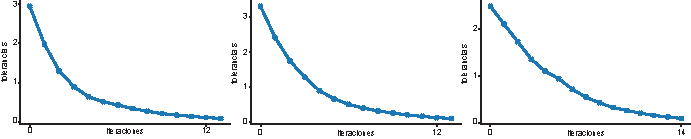
\includegraphics[width=1\columnwidth]{figures/chapter7/C7_eps.pdf} 
    \caption{\textbf{Convergencia del Cálculo Bayesiano Aproximado Monte Carlo Secuencial}. Evolución de la tolerancia a medida que aumentan las iteraciones para el modelo de las secciones \ref{C7_sec:OU} (izquierda),  \ref{C7_sec:OUD} (centro) y  \ref{C7_sec:dist} (derecha).}
    \label{C7_fig:ap_eps}
\end{figure} 


Los 1000 parámetros aceptados por el ABC-SMC y sus respectivos pesos se encuentran en \href{https://github.com/fiorefabris/parameters}{\underline{este link}}. En cada caso, se encuentra marcado en rojo los parámetros que utilizamos para ejemplificar los resultados de cada ajuste.

Las series temporales surgidas del conjunto de parámetros que elegimos para validar el modelo, así como el resultado del algoritmo de detección de pulsos se encuentran en las figuras \ref{C6_ap_fig:traces_evaluation} (sección \ref{C6_sec:alder_ruido_fit}), \ref{C7_fig:OU_traces_VM} (sección \ref{C7_sec:OU}), \ref{C7_fig:OUD_traces_VM} (sección \ref{C7_sec:OUD}) y \ref{C7_fig:dist_traces_VM} (sección \ref{C7_sec:dist}) . Decidimos en este caso visualizar las series temporales a partir del observable 
\begin{equation}
    s(t) = \frac{e^{k\sin{(\theta(t))}}}{e^{k}},
    \label{C7_eq:VM}
\end{equation}
donde elegimos k = 100. Con esta transformación, es más sencillo distinguir a simple vista las excursiones de la fase del ruido de fondo. Esta ventaja es en detrimento de (i) utilizar una expresión más compleja que la de la ecuación \ref{C5_eq:seno_fase}, y (ii) que las excursiones de la fase en sentido horario, que en esta tesis no consideramos como pulsos, también son más fáciles de distinguir a simple vista y más difíciles de distinguir de las excursiones en sentido antihorario, o pulsos. 


\begin{figure}
    \centering
    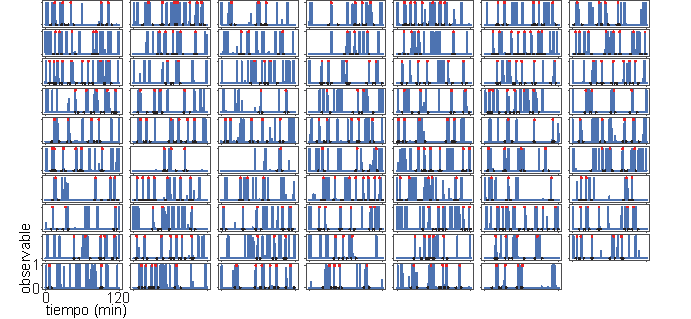
\includegraphics[width=1\columnwidth]{figures/chapter6/C6_traces_for_evaluation_VM.pdf} 
    \caption{\textbf{Series temporales sintéticas y detección de pulsos para analizar el modelo de fase con bifurcación de ciclo infinito y ruido blanco gaussiano aditivo.} Series temporales del observable \ref{C7_eq:VM} de la fase en función del tiempo para el modelo \ref{C6_eq:adler_white_noise}. Se encuentra también representado el resultado del algoritmo de detección de pulsos, donde el inicio (triángulo negro con el vértice del lado izquierdo), el pico (rojo) y el final (triángulo negro con el vértice del lado derecho) de cada pulso detectado están indicados. Los picos observados que no fueron identificados como pulsos son, en su mayoría, excursiones de la fase en sentido horario. Parámetros:  $\omega = 0.33\;\text{min}^{-1}$, $\alpha = 1.02 \times \omega$, $ D = 0.43 \;\text{min}^{-2}$. La tasa de adquisición fue de $dt = 0.001$, cada $d = 1$ pasos. El umbral de amplitud del algoritmo de detección de pulsos fue $A_{\text{th}} = 0.9$, y la distancia umbral fue de $W_{\text{th}} = 100\text{ cuadros}$. N = $69$ series temporales. $T = 120$ minutos de duración.}
    \label{C6_ap_fig:traces_evaluation}
\end{figure}


\begin{figure}
    \centering
    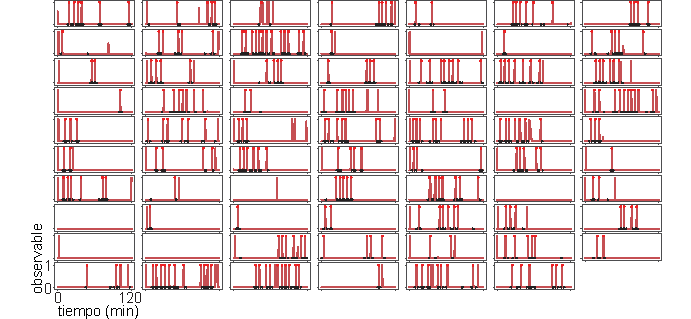
\includegraphics[width=1\columnwidth]{figures/chapter7/C7_OU_traces_for_evaluation_VM.pdf} 
    \caption{\textbf{Series temporales sintéticas y detección de pulsos para explorar el modelo de fase con bifurcación de ciclo infinito y amplitud de modulación como proceso de Ornstein-Uhlenbeck.} Series temporales del observable \ref{C7_eq:VM} de la fase en función del tiempo para el modelo de la sección \ref{C7_sec:OU}. Se encuentra también representado el resultado del algoritmo de detección de pulsos, donde el inicio (triángulo negro con el vértice del lado izquierdo), el pico (rojo) y el final (triángulo negro con el vértice del lado derecho) de cada pulso detectado están indicados. Los picos observados que no fueron identificados como pulsos son, en su mayoría, excursiones de la fase en sentido horario. Parámetros: $\omega = 1.11\;\text{min}^{-1}$, $\alpha_0 = 1.23 \times \omega$, $ \sigma = 2.94 \; \;\text{min}^{-3/2}$ y $\tau = 61.02 \; \text{min} $. La tasa de adquisición fue de $dt = 0.001$, cada $d = 1$ pasos. El umbral de amplitud del algoritmo de detección de pulsos fue $A_{\text{th}} = 0.9$, y la distancia umbral fue de $W_{\text{th}} = 100\text{ cuadros}$. N = $69$ series temporales. $T = 120$ minutos de duración.}
    \label{C7_fig:OU_traces_VM}
\end{figure}

 
\begin{figure}
    \centering
    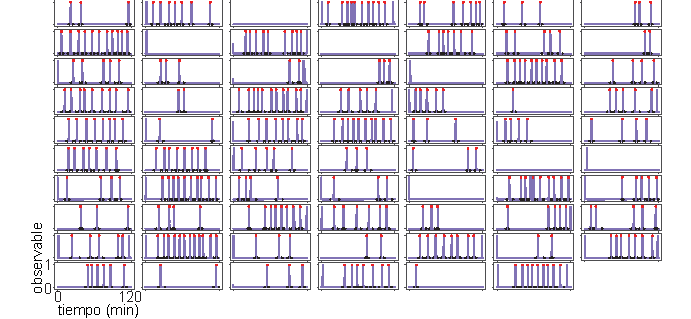
\includegraphics[width=1\columnwidth]{figures/chapter7/C7_OUD_traces_for_evaluation_VM.pdf} 
    \caption{\textbf{Series temporales sintéticas y detección de pulsos para explorar el modelo de fase con bifurcación de ciclo infinito, amplitud de modulación como proceso de Ornstein-Uhlenbeck y ruido blanco gaussiano aditivo.} Series temporales del observable \ref{C7_eq:VM} de la fase en función del tiempo para el modelo de la sección \ref{C7_sec:OUD}. Se encuentra también representado el resultado del algoritmo de detección de pulsos, donde el inicio (triángulo negro con el vértice del lado izquierdo), el pico (rojo) y el final (triángulo negro con el vértice del lado derecho) de cada pulso detectado están indicados. Los picos observados que no fueron identificados como pulsos son, en su mayoría, excursiones de la fase en sentido horario. Parámetros: $\omega = 0.65 \;\text{min}^{-1}$, $\alpha_0 = 1.08 \times \omega$, $ \sigma = 0.45 \;\text{min}^{-3/2}$, $\tau = 142.06 \; \text{min} $ y $D = 0.11 \;\text{min}^{-2}$. La tasa de adquisición fue de $dt = 0.001$, cada $d = 1$ pasos. El umbral de amplitud del algoritmo de detección de pulsos fue $A_{\text{th}} = 0.9$, y la distancia umbral fue de $W_{\text{th}} = 100\text{ cuadros}$. N = $69$ series temporales. $T = 120$ minutos de duración.}
    \label{C7_fig:OUD_traces_VM}
\end{figure}

\begin{figure}
    \centering
    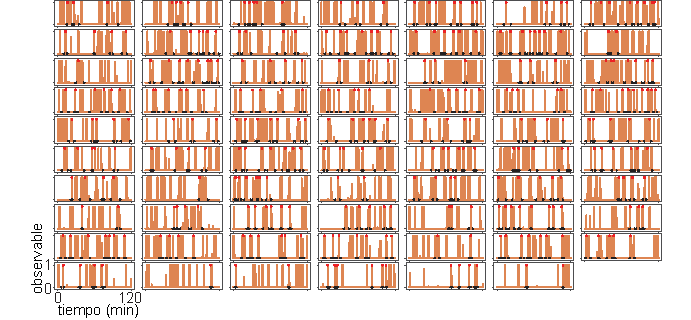
\includegraphics[width=1\columnwidth]{figures/chapter7/C7_dist_traces_for_evaluation_VM.pdf} 
    \caption{\textbf{Series temporales sintéticas y detección de pulsos para explorar el modelo de fase con bifurcación de ciclo infinito, ruido blanco gaussiano aditivo y variabilidad en la amplitud de modulación estacionaria.} Series temporales del observable \ref{C7_eq:VM} de la fase en función del tiempo para el modelo de la sección \ref{C7_sec:OUD}. Se encuentra también representado el resultado del algoritmo de detección de pulsos, donde el inicio (triángulo negro con el vértice del lado izquierdo), el pico (rojo) y el final (triángulo negro con el vértice del lado derecho) de cada pulso detectado están indicados. Los picos observados que no fueron identificados como pulsos son, en su mayoría, excursiones de la fase en sentido horario. Parámetros: $\omega = 0.30 \; \text{min}^{-1}$, $\mu_{\alpha} = 0.06 \times \omega$, $ \sigma_{\alpha} = 0.36  \times \omega$ y $D = 0.54 \; \text{min}^{-2}$. La tasa de adquisición fue de $dt = 0.001$, cada $d = 1$ pasos. El umbral de amplitud del algoritmo de detección de pulsos fue $A_{\text{th}} = 0.9$, y la distancia umbral fue de $W_{\text{th}} = 100\text{ cuadros}$. N = $69$ series temporales. $T = 120$ minutos de duración.}
    \label{C7_fig:dist_traces_VM}
\end{figure}
\end{subappendices}

\end{document}